\chapter{Background}\label{chap:background}
The following work is based on the book Reinforcement Learning:
An Introduction\cite{Sutton1998} from Richard S. Sutton and Andrew G. Barto
\section{Markov Decision Processes}
The Markov Decision Process (MPD)  is the mathematical framework of Reinforcement Learning and
is defined as a tuple < $\mathcal{S, A, R, T, }$ >
\begin{itemize}
\item $\mathcal{S}$ is a number of states, s $\in \mathcal{R}^{n}$
\item $\mathcal{A}$ is a of actions, a $ \in \mathcal{R}^{n}$
\item $\mathcal{T}$ is the transition probability function
\item $\mathcal{R}$ is the reward
\end{itemize}


Every state in a Markov Decision Process needs satisfy the Markov Property.
This means that "The future is independent of the past given the present".
The definition is given by an State Reward pair as 


\begin{equation}
\mathcal{P}(S_{t+1}, R_{t+1}) | S_{t}, R_{t}) =  \mathcal{P}(S_{t+1}, R_{t+1}) | S_{t+1}, R_{t+1}, S_{t+1}, R_{t+1})
\end{equation}

Unfortunately for most real-world problem this assumption is violated. This is also the case for the
state transition function, which is definite as

\begin{equation}
  \mathcal{P}(S_{t+1}| R_{t+1}) | s_{t}, a_{t}) =  \mathcal{P}(S_{t+1}| S_{t} = s ,  A_{t} = a)
\end{equation}
 
The Reward is a function of state action pairs
\begin{equation}
  \mathcal{P}(S_{t+1}| R_{t+1}) | s_{t}, a_{t}) =  \mathcal{P}(S_{t+1}| S_{t} = s ,  A_{t} = a)
\end{equation}
 
The goal of the agent is to find the policy that maximizes the total reward.
This policy is a function that maps states to actions in the deterministic case.
While a stochastic policy has a certain probability to choose an action in a state.
For any MDP there is always at least one optimal policy. 
In case the transition probability is given, the dynamic programming-based Value Iteration  Algorithm is one way to compute this policy.
Which is build upon the concept of a Value Function.


\subsection{Value Function}
The value function $V^{\pi}$ : $\mathcal{S}$ $\rightarrow$ $\mathcal{R}$, represents expeceted total reward of a policy in a given state and following the policy
It is defined as follows,
 
\begin{equation}
  \begin{aligned}
    V^{\pi}(s) &= \mathbb{E}_{\pi} [R_t | s_t = s] \\
    &= \mathbb{E}_{\pi} [\sum^{\infty}_{k=0} \gamma^{k} r_{t+k+1} | s_t = s] \label{MDP:eq1} \\
    &= \sum_{a \in \mathcal{A}} \pi(s, a) \sum_{s' \in \mathcal{S}} \mathcal{T}^{a}_{ss'}[\mathcal{R}^{a}_{ss'} + \gamma V^\pi(s')]
  \end{aligned}
\end{equation}


One way to find the optimal policy is the value Iteration Algorithm.
In each Iteration the value function is updated by the following equation,

\begin{equation}
  V_{i+1}(s) := \max_a \Big\{ \sum_{s', r} P(s',r| s,a) (r + \gamma V_i(s')) \Big\}
\end{equation}


\subsection{Q Function}

In many real-world problems, the transition function is unknown, and approximate the Value function is not feasible, because
it would require evaluating all possible actions in a single state every time step.
In this case the Q-value function helps by using the state action pair


\begin{equation}
  Q(s_t, a_t) \leftarrow Q(s_t, a_t) + \alpha[r_{t+1} + \gamma \max_a Q(s_{t+1}, a) - Q(s_t, a_t)]
\end{equation}


This update equation is used to find an optimal policy in the Q-Learning Algorithm, repesened in Algorithm \ref{alg:q-learning}

\begin{algorithm}[H]
\caption{Q-learning}
\label{alg:q-learning}
\begin{algorithmic}
    \State Algorithm parameters: learning rate $\alpha \in (0, 1]$, discount factor $\gamma \in (0, 1]$, exploration rate $\epsilon > 0$
    \State Initialize $Q(s,a)$ randomly except $Q(terminal, \cdot) = 0$
    \While{not converges}
        \State Set initial state $s$  
        \While{$s$ is not terminal}
            \State With probability $\epsilon$:
            \State \hspace{\algorithmicindent} Pick random action $a$
            \State otherwise:
            \State \hspace{\algorithmicindent} $a$ = argmax$_a$ $Q(s, a)$
            \State Execute action $a$ and observe reward $r$ and succesor state $s'$
            \State$Q(s, a) \leftarrow Q(s, a) + \alpha[r + \gamma \max_{a^*} Q(s', a^*) - Q(s, a)]$
            \State $s \leftarrow s'$
        \EndWhile
    \EndWhile
\end{algorithmic}
\end{algorithm}



The fact that the policy for interacting with the environment is different from the one to update the Q-value Function makes it to an off-policy Algorithm


\section{Neural Network}

In complex environments, the state space is continuous, which makes it infeasible to use to store all state-action pairs in a table.
Advances in machine learning especially in deep learning make it possible to approximate this Q function.  
A basic element of Deep learning is artificial neural networks which are inspired by the human brain.
Neural network have a structure of input layer connected to hidden layers followed by the output layer. 
A standard Network has linear many hidden layers represented as nodes. The nodes between different layers are connected by weights. 
The values of the weights can be trained iteratively by using an optimization  technique like stochastic gradient descent and backpropagation.
This simple architecture could be seen as matrix multiplications which makes it a linear function. 
By adding nonlinear activation functions it is able to approximate more complex nonlinear functions.


\begin{figure}[h]
  \centering
  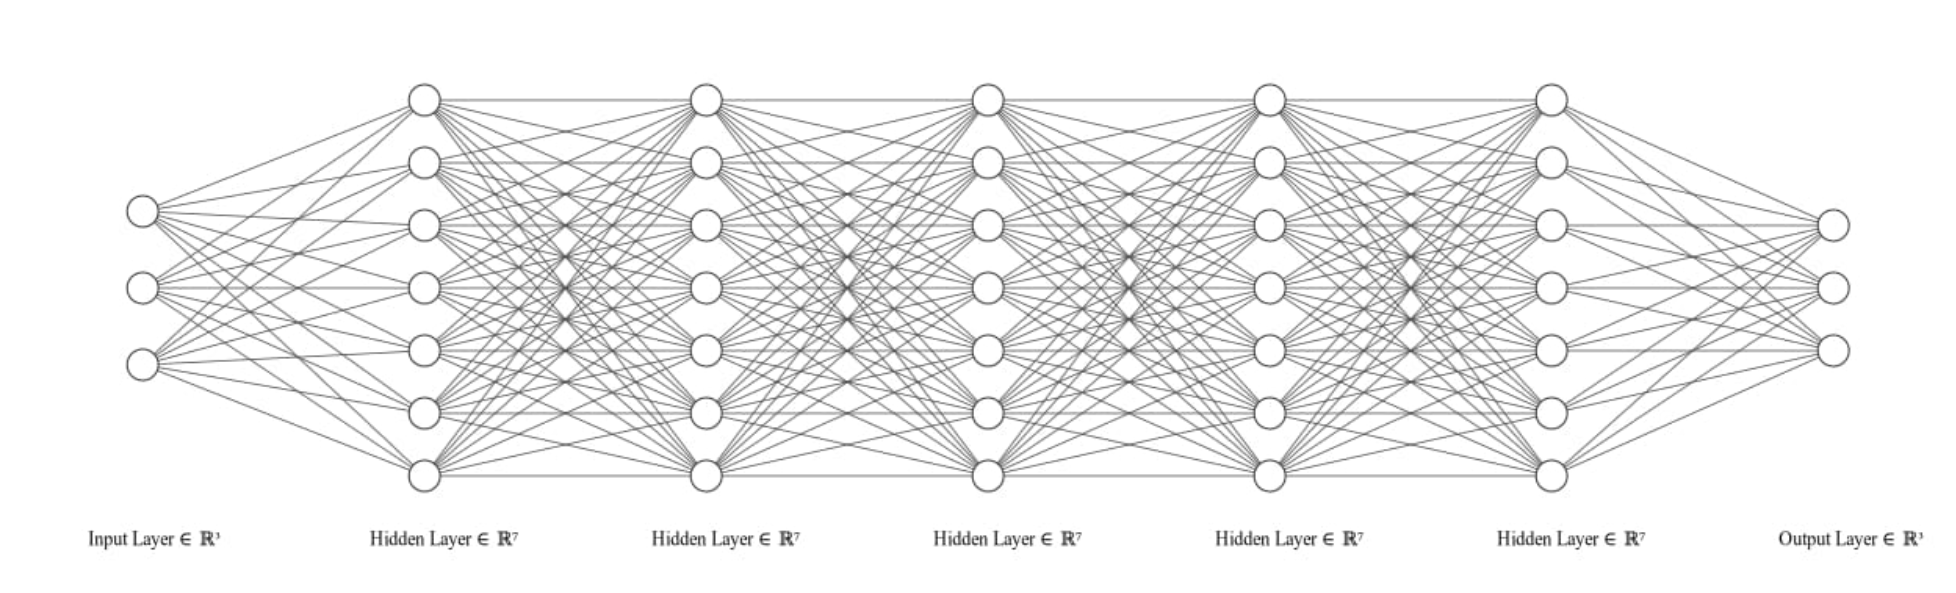
\includegraphics[width=0.5\textwidth]{figures/background/nn.png}
  \caption{Deep Neural Network with several hidden layers}
  \label{fig:tab-training}
\end{figure}


